% Optional figure blocks: copy to the desired locations in the report.
% The current report does not input this file automatically.
% Both PDFs use the exact exported target of connectivity_linear.pdf.

\begin{figure}[!ht]
  \centering
  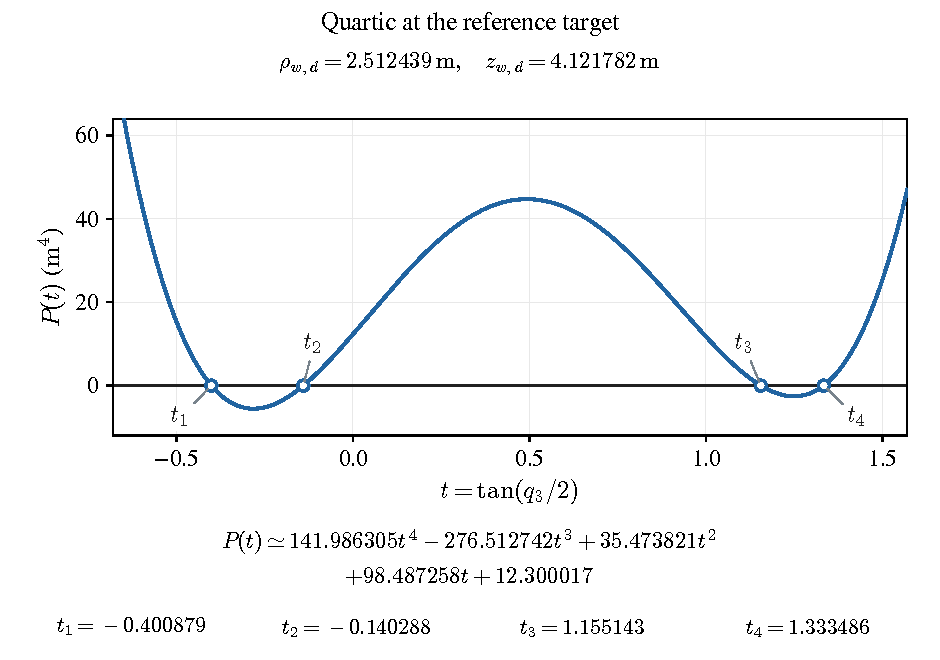
\includegraphics[width=\linewidth]{figures/connectivity_quartic.pdf}
  \caption{The arm IK quartic at the reference target of the connectivity
  example, with $t=\tan(q_3/2)$. Its four distinct real roots are labelled
  in increasing order, consistently with the joint-space and workspace maps.
  Each root determines one arm solution; the two wrist branches share the
  same arm root. The plotted polynomial uses the full-precision target;
  displayed coefficients and root values are rounded.}
  \label{fig:connectivity-quartic}
\end{figure}

\begin{figure}[!ht]
  \centering
  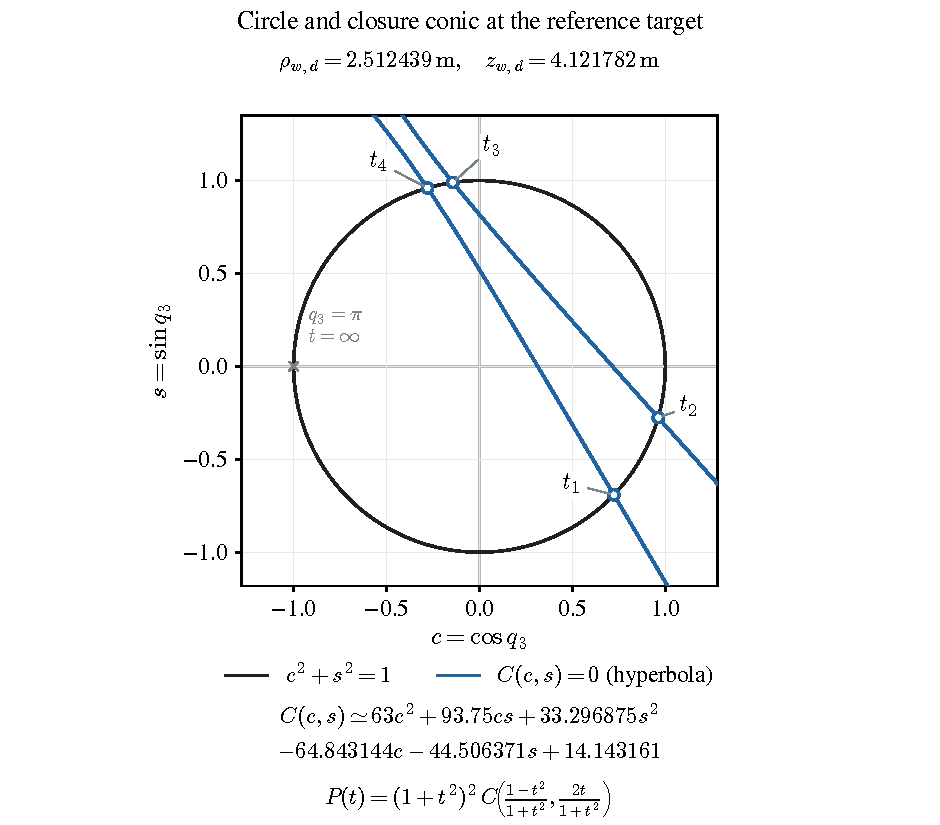
\includegraphics[width=\linewidth]{figures/connectivity_circle_conic.pdf}
  \caption{The same four arm solutions as intersections of the unit circle
  with the closure conic $C(c,s)=0$, where $c=\cos q_3$, $s=\sin q_3$,
  and $C(\cos q_3,\sin q_3)=c_\gamma^2G(q_3)$.
  Here the conic is a hyperbola. The labels $t_i$ identify the same roots as
  in the quartic plot; their counterclockwise cyclic order is
  $t_1,t_2,t_3,t_4$, with $t_4$ adjacent to $t_1$ across the angular seam.
  The grey cross marks the omitted half-angle point $q_3=\pi$
  ($t=\infty$), which is not a root for this target.}
  \label{fig:connectivity-circle-conic}
\end{figure}
